\documentclass[11pt]{article}

% ---------- Packages ----------
\usepackage[utf8]{inputenc}
\usepackage[T1]{fontenc}
\usepackage{lmodern}                 % cleaner default font
\usepackage[margin=1in]{geometry}    % sane margins
\usepackage{graphicx}                % images
\usepackage{subcaption}
\usepackage{amsmath,amssymb,amsthm}  % core math
\usepackage{mathtools}               % \coloneqq, better cases, etc.
\usepackage{bm}                      % bold math symbols (vectors)
\usepackage{booktabs}                % nice tables
\usepackage{caption}
\usepackage{enumitem}
\usepackage{xcolor}
\usepackage[colorlinks=true,linkcolor=blue,citecolor=blue,urlcolor=blue]{hyperref}
\usepackage{cleveref}                % \cref smart references (load after hyperref)
\usepackage[numbers,sort&compress]{natbib}  % numbered [1] citations, merges ranges

% ---------- Spacing / readability ----------
\setlength{\parskip}{0.5em}
\setlength{\parindent}{0pt}
\renewcommand{\arraystretch}{1.2}

% ---------- Theorem-like environments ----------
\theoremstyle{definition}
\newtheorem{definition}{Definition}[section]
\newtheorem{remark}{Remark}[section]

% ---------- Custom shortcuts ----------
\renewcommand{\Re}{\operatorname{Re}}
\renewcommand{\Im}{\mathfrak{Im}}

% ---------- Title ----------
\title{LSU REU Code Documentation}
\author{Idden Tsai}
\date{Summer 2026}
\begin{document}

\maketitle

\begin{abstract}
\noindent
Mathematical documentation and numerical derivations for the time-dependent Ginzburg--Landau (TDGL) solver developed during the LSU REU, replicating the vortex-dynamics results of Embon \textit{et al.}~\cite{embon2017}.
\end{abstract}

\tableofcontents

\newpage

% ================================================================

\section{Introduction}
\label{sec:intro}

\subsection{Governing Equations}
\label{sec:governing-equations}

\begin{equation}
\label{eq:tdgl-psi}
\frac{u}{\sqrt{1 + \gamma^2 |\psi|^2}} \left( \frac{\partial}{\partial t} + i \phi + \frac{\gamma^2}{2} \frac{\partial |\psi|^2}{\partial t} \right) \psi = (\nabla - i A)^2 \psi + (1 - |\psi|^2) \psi
\end{equation}

\begin{equation}
\label{eq:tdgl-phi}
\sigma_n \nabla^2 \phi = \nabla \cdot \Im\!\left\{ \psi^* (\nabla - i A) \psi \right\}
\end{equation}

\begin{equation}
\label{eq:tdgl-ampere}
\kappa^2 \, \nabla \times \nabla \times A = J_s + J_n
\end{equation}

These are the three coupled equations my code uses to solve for the time evolution of the order parameter ($\psi$), the electrostatic potential ($\phi$), and the magnetic vector potential (A). The constants are defined as $u = 5.79$, $\gamma = 0$, $\sigma_n = 1$, and $\kappa = 2.1$. $\gamma$ is set to zero throughout and the derivations keep it for generality. The choice of $\kappa$ arises from Embon \textit{et al.}~\cite{embon2017}, which uses an experimental $\lambda = 96\,\text{nm}$ and $\xi = 46\,\text{nm}$, resulting in $\kappa \approx 2.1$.

\subsection{Boundary Conditions}
\label{sec:bc}

$\hat{n}$ is defined as the unit vector perpendicular to the superconducting boundary.
No supercurrent leaves the boundary.

\begin{equation}
\label{eq:bc-super}
\hat{n} \cdot (\nabla - i A) \psi = 0
\end{equation}

No normal current leaves the boundary.

\begin{equation}
\label{eq:bc-normal}
\hat{n} \cdot \nabla \phi = 0
\end{equation}

Current injection. Positive $J_{inj}$ is in the $+\hat{x}$ direction.

\begin{equation}
\label{eq:bc-inject}
\sigma_n \nabla \phi = J_{\mathrm{inj}}
\end{equation}

\subsection{Dimensionless Scaling}
\label{sec:scaling}

All scaling procedures follow Embon \textit{et al.}~\cite{embon2017}, but I will define them here for clarity, as a few suspected typos in that paper may become sources of confusion.
Below are the constants used in the scaling equations in SI units:

\begin{equation}
\label{eq:scale-constants}
\xi = 46\,\text{nm} \qquad \lambda = 96\,\text{nm} \qquad T = 4.2\,\text{K} \qquad T_c = 7.2\,\text{K}
\end{equation}

\begin{equation}
\label{eq:scale-AB}
A_0 = \frac{\Phi_0}{2 \pi \xi} \qquad B_0 = \frac{\Phi_0}{2 \pi \xi^2} \approx 155\,\text{mT}
\end{equation}

\begin{equation}
\label{eq:scale-tau}
\tau_{\mathrm{GL}} = \frac{\pi \hbar}{8 k_B T_c \left( 1 - \frac{T}{T_c} \right) u} \approx 1.73 \times 10^{-13}\,\text{s}
\end{equation}

\begin{equation}
\label{eq:scale-phi}
\phi_0 = \frac{\hbar}{e^* \tau_{\mathrm{GL}}} \approx 1.9\,\text{mV}
\end{equation}

\begin{equation}
\label{eq:scale-Jn}
J_{n,\mathrm{GL}} = \frac{\sigma_n \Phi_0}{2 \pi \xi \tau_{\mathrm{GL}}} = \tilde{\sigma}_n J_{s,\mathrm{GL}}
\end{equation}

\subsection{Parameter (In Code) Definitions}
\label{sec:params}

\begin{description}[leftmargin=!,labelwidth=6em,style=nextline,itemsep=0.2em]
  \item[dimx] the number of grid points in the x-direction
  \item[dimy] the number of grid points in the y-direction
  \item[n] the total number of grid points in the superconducting domain
  \item[nA] the total number of grid points in the vacuum domain
  \item[ymax] the vertical size of the system in coherence lengths ($\xi$)
  \item[h] defined as ymax / (dimy-1)
  \item[n\_t] the number of time steps
  \item[tmax] the total number of dimensionless time units in $\tau_{\mathrm{GL}}$
  \item[dt] defined as tmax / n\_t
  \item[n\_relax] the number of time steps where current is zero at the beginning
  \item[n\_ramp] the number of time steps the current ramps over after n\_relax
  \item[H\_relax] the number of time steps the external magnetic field is zero at the beginning
  \item[H\_ramp] the number of time steps the external magnetic field ramps over after H\_relax
  \item[stride] the number of time steps between each .bin save (excluding power.bin)
  \item[stride\_power] the number of time steps between each power.bin save
  \item[stride\_mumps] the number of time steps between each \cref{eq:tdgl-phi} solve
  \item[H\_ext] the maximum value the externally applied magnetic field ramps to
  \item[current\_max] the maximum value the current ramps to
  \item[print\_stride] the number of time steps between each diagnostic print
\end{description}

% ================================================================

\section{Equations and Derivations}
\label{sec:derivations}

\subsection{Forward Euler}
\label{sec:forward-euler}

\begin{equation}
\label{eq:fe-rearranged}
\frac{\sqrt{1 + \gamma^2 |\psi|^2}}{u} \left( (\nabla -iA)^2 \psi + (1 - |\psi|^2) \psi \right) - i \phi \psi = \frac{\partial \psi}{\partial t} + \frac{\gamma^2}{2} \frac{\partial |\psi|^2}{\partial t} \psi
\end{equation}

First, isolate the time derivative terms in \cref{eq:tdgl-psi} obtaining \cref{eq:fe-rearranged} to prepare for some algebra as the $\frac{\partial |\psi|^2}{\partial t}$ term poses a challenge to using forward Euler.

\begin{equation}
\label{eq:dt-modsq}
\partial_t (\psi^* \psi) = (\partial_t \psi^*) \psi + \psi^* (\partial_t \psi) = z^* + z = 2\Re(z) = 2\Re(\psi^* \partial_t \psi)
\end{equation}

where $z = \psi^* (\partial_t \psi)$. You can then plug this result into the RHS of \cref{eq:fe-rearranged} to obtain

\begin{equation}
\label{eq:rhs-sub}
\partial_t \psi + \gamma^2 \Re(\psi^* \partial_t \psi) \psi.
\end{equation}

We define $X = \partial_t \psi$, $S = \Re(\psi^* X)$, and G as the LHS of \cref{eq:fe-rearranged}.

\begin{align}
G &= X + \gamma^2 S \psi \label{eq:G-def}\\
X &= G - \gamma^2 S \psi \label{eq:X-def}\\
\psi^* X &= \psi^* G - \psi^* \psi \gamma^2 S \label{eq:psiX}\\
\Re(\psi^* X) &= \Re(\psi^* G) - |\psi|^2 \gamma^2 S \label{eq:RepsiX}\\
S + |\psi|^2 \gamma^2 S &= \Re(\psi^* G) = S (1 + |\psi|^2 \gamma^2) \label{eq:Ssum}\\
S &= \frac{\Re(\psi^* G)}{1 + |\psi|^2 \gamma^2} \label{eq:S-result}
\end{align}

With this, we can substitute $S$ and $X$ back into \cref{eq:X-def} to obtain

\begin{equation}
\label{eq:X-result}
X = G - \gamma^2 \psi \frac{\Re(\psi^* G)}{1 + |\psi|^2 \gamma^2} = \partial_t \psi.
\end{equation}

Now that we have isolated the time derivative, the time step equation looks like this

\begin{equation}
\label{eq:psi-timestep-naive}
\psi^{n+1} = \psi^n + \Delta t \Big[ G^n - \frac{\gamma^2 \psi^n}{1 + |\psi^n|^2 \gamma^2} \Re\big( (\psi^n)^* G^n \big) \Big] \quad G^n = \frac{\sqrt{1 + \gamma^2 |\psi^n|^2}}{u} \left( (\nabla - iA)^2 \psi^n + (1 - |\psi^n|^2) \psi^n \right) - i \phi \psi^n
\end{equation}

A problem arises with this time step formula. The $-i \phi \psi$ term is unconditionally unstable for Forward Euler. Just take the $- i \phi \psi$ term and look at its relationship with the time derivative.

\begin{align}
\frac{\psi^{t+1} - \psi^t}{\Delta t} &= -i \phi \psi \label{eq:phi-instab}\\
\psi^{t+1} &= \psi^t (1 - i \phi \Delta t) \label{eq:phi-amp}
\end{align}

The amplification factor is

\begin{equation}
\label{eq:amp-factor}
|1 - i \phi \Delta t| = \sqrt{1 + (\phi \Delta t)^2}
\end{equation}

which for any $\Delta t > 0$ and $\phi \neq 0$ is greater than 1.
So instead of letting this happen, I use an integrating factor to get rid of this term.

\begin{equation}
\label{eq:N-def}
\mathcal{N}(\psi^t) = G_{\mathrm{rest}}^t - \frac{\gamma^2 \psi^t}{1 + |\psi^t|^2 \gamma^2} \Re\big( (\psi^t)^* G_{\mathrm{rest}}^t \big) \qquad G_{\mathrm{rest}}^t = \frac{\sqrt{1 + \gamma^2 |\psi^t|^2}}{u} \left( (\nabla - iA)^2 \psi^t + (1 - |\psi^t|^2) \psi^t \right)
\end{equation}

The rest of the proof is below. Also, from here on dt will replace $\Delta t$.

\begin{align}
\partial_t \psi &= -i \phi \psi + \mathcal{N}(\psi) \label{eq:dpsi-split}\\
\psi(t) &= e^{-i \phi t} \chi(t) \label{eq:chi-sub}
\end{align}

Where $\chi(t)$ is currently unknown, but we can take the derivative of the equation just above to obtain

\begin{equation}
\label{eq:dchi}
\partial_t \psi = -i \phi e^{-i \phi t} \chi(t) + e^{-i \phi t} \partial_t \chi
\end{equation}

Now you may have noticed that $\phi$ here is constant even when it evolves in time. I will be treating this as an approximation that will introduce some first-order error.

We can then set the equation above equal to the first time derivative of the form $\partial_t \psi = -i \phi \psi + \mathcal{N}(\psi)$.

\begin{align}
-i \phi e^{-i \phi t} \chi(t) + \mathcal{N}(e^{-i \phi t} \chi(t)) &= -i \phi e^{-i \phi t} \chi(t) + e^{-i \phi t} \partial_t \chi \label{eq:setequal}\\
\mathcal{N}(e^{-i \phi t} \chi(t)) &= e^{-i \phi t} \partial_t \chi \label{eq:setequal2}\\
e^{i \phi t} \mathcal{N}(e^{-i \phi t} \chi(t)) &= \partial_t \chi \label{eq:dchi-dt}
\end{align}

With this definition for the time derivative of $\chi(t)$, we can set up the equation.

\begin{equation}
\label{eq:chi-integral}
\chi(dt) = \chi(0) + \int_0^{dt} e^{i \phi s} \mathcal{N}(e^{-i \phi s} \chi(s)) \, ds
\end{equation}

We will use the the Taylor series and $f(s) = e^{i \phi s} \mathcal{N}(\psi(s))$.

\begin{align}
f(s) &\approx f(0) + f'(0) s + f''(0) \frac{s^2}{2} \cdots \label{eq:taylor-f}\\
\int_0^{dt} f(s) \, ds &= f(0) dt + f'(0) \frac{dt^2}{2} \cdots \label{eq:taylor-int}
\end{align}

However, for the next step, only retain the first term in the Taylor series expansion, which will result in some global first-order error $\mathcal{O}(dt)$. However, this is not a significant problem, considering that Forward Euler error is already first order error.

\begin{equation}
\label{eq:integral-approx}
\int_0^{dt} e^{i \phi s} \mathcal{N}(\psi(s)) \, ds \approx e^{i \phi 0} \mathcal{N}(\psi(0)) dt \approx \mathcal{N}(\psi(0)) dt
\end{equation}

Now we can plug this approximated integral back into \cref{eq:chi-integral} with $\chi(0) = \psi(0)$.

\begin{equation}
\label{eq:chi-dt-approx}
\psi(0) + \int_0^{dt} e^{i \phi s} \mathcal{N}(\psi(s)) \, ds \approx \psi(0) + \mathcal{N}(\psi(0)) dt \approx \chi(dt)
\end{equation}

Look back at \cref{eq:chi-sub} and plug in dt into t and the $\chi(dt)$ solved for just above.

\begin{align}
\psi(dt) &= e^{-i \phi dt} \chi(dt) \label{eq:psi-dt}\\
\psi_{\mathrm{new}} &= e^{-i \phi dt} \big( \psi_{\mathrm{old}} + \mathcal{N}(\psi_{\mathrm{old}}) dt \big) \label{eq:psi-new}
\end{align}

The reason we can call $\psi(dt) = \psi_{\mathrm{new}}$ and $\psi(0) = \psi_{\mathrm{old}}$ is that we can just treat 0 as any time reference point and dt as just the small step we take to get to the next point. This is taken into account via the integral, so $\psi(0)$ can really just start anywhere.

In conclusion, the Forward Euler equation I use in the code is this.

\begin{equation}
\label{eq:fe-final}
\psi^{t+1} = e^{-i \phi \Delta t} (\psi^t + \Delta t \mathcal{N}(\psi^t)) \qquad \mathcal{N}(\psi^t) = G_{\mathrm{rest}}^t - \frac{\gamma^2 \psi^t}{1 + |\psi^t|^2 \gamma^2} \Re\big( (\psi^t)^* G_{\mathrm{rest}}^t \big)
\end{equation}

\begin{equation}
\label{eq:Grest-final}
G_{\mathrm{rest}}^t = \frac{\sqrt{1 + \gamma^2 |\psi^t|^2}}{u} \left( (\nabla - iA)^2 \psi^t + (1 - |\psi^t|^2) \psi^t \right)
\end{equation}

Note for \cref{eq:fe-final}, if $\gamma = 0$, $\mathcal{N}(\psi^t) = G_{\mathrm{rest}}^t.$

\subsection{Constriction}
\label{sec:constriction}

The function below is the equation I used to create the non-superconducting regions, the constriction, in the simulation. See Embon \textit{et al.}'s supplementary notes for more details~\cite{embon-supps}.

\begin{equation}
\label{eq:constriction}
\left| l_{\mathrm{half}} - \frac{(l_{\mathrm{half}} - w_{0,\mathrm{half}})}{1 + (\frac{x}{R})^2} \right| < y
\end{equation}

$l_{\mathrm{half}}$ is defined as the vertical half-width of the widest region (left and right) of the superconducting passage.

$w_{0,\mathrm{half}}$ is defined as the half-width of the thinnest region (the constriction) in the passage.

The $x$ values are represented by the variable $\texttt{j}$ and the $y$ values use variable $\texttt{i}$. R is the radius of the constriction.

\subsection{Supercurrent}
\label{sec:supercurrent}

I represented the supercurrent and the rest of the vector values in my code on a staggered grid where vectors lie between grid points (nodes) instead of on the nodes. See~\cref{sec:staggered-grid} for reasoning.

\begin{equation}
\label{eq:Js-analytic}
J_s = \Im\!\left\{ \psi^* (\nabla - i A) \psi \right\}
\end{equation}

We can discretize this first.

\begin{equation}
\label{eq:Js-disc}
J_s = \Im\!\left\{ \psi^*_i \frac{U_i \psi_{i+1} - \psi_i}{h} \right\}
\end{equation}

Since $\psi^*_i \psi_i$ is real we can cancel it from the Im.

\begin{equation}
\label{eq:Js-disc-final}
= \frac{1}{h} \Im\!\left\{ \psi^*_i U_i \psi_{i+1} \right\}
\end{equation}

where $U_i$ is the link variable between $\psi_{i+1}$ and $\psi_i$.

\subsection{Divergence of the Supercurrent}
\label{sec:div-js}

\begin{equation}
\label{eq:divJs-analytic}
\nabla \cdot J_s = \nabla \cdot \Im\!\left\{ \psi^* (\nabla - i A) \psi \right\}
\end{equation}

The formula above is the analytical equation for solving for the divergence of the supercurrent. Since I'm doing things on a computer let's derive a discretized version with link variables.

\begin{align}
\nabla \cdot J_s &= \nabla \cdot \Im\!\left\{ \psi^* (\nabla - i A) \psi \right\} \label{eq:divJs-1}\\
&= \nabla \cdot \Im\!\left\{ \psi^*_x \frac{U_x \psi_{x+1} - \psi_x}{h} \right\} \label{eq:divJs-2}\\
&= \nabla \cdot \frac{1}{h} \Im\!\left\{ \psi^*_x U_x \psi_{x+1} \right\} \label{eq:divJs-3}\\
&= \frac{1}{h} \left( \frac{\Im\!\left\{ \psi^*_x U_x \psi_{x+1} \right\} - \Im\!\left\{ \psi^*_{x-1} U_{x-1} \psi_x \right\}}{h} \right) \label{eq:divJs-4}
\end{align}

Now we use the identity $\Im\!\left\{ z \right\} = -\Im\!\left\{ z^* \right\}$.

\begin{align}
&= \frac{1}{h^2} \big( \Im\!\left\{ \psi^*_x U_x \psi_{x+1} \right\} + \Im\!\left\{ \psi_x^* U_{x-1}^* \psi_{x-1} \right\} \big) \label{eq:divJs-final}
\end{align}

This is the equation I use for the divergence of $J_s$. An important specification is that the $A_x$ term in the exponential of the link variable is the vector potential between the two $\psi$'s, which is on the staggered grid~\ref{sec:staggered-grid}. Also, instead of using an integral in the link variable~\ref{sec:link-variables}, I use the approximation of small h to treat $A_x$ as constant, resulting in $U_x = e^{-i A_x h}$. Using the $A_x$ on the staggered grid between $\psi$'s reduces the error of this approximation as well.

\subsection{Poisson Solve}
\label{sec:poisson}

To solve \cref{eq:tdgl-phi}, you must first set up the Laplacian matrix ($L$) in the code.

\begin{equation}
\label{eq:Lphib}
L \phi = b
\end{equation}

However, $L$ is singular meaning there is no unique solution to $\phi$ unless $b = \frac{\nabla \cdot J_s}{\sigma_n}$ is orthogonal to the non-zero null space vector. It is also symmetric.
Here is a quick justification for the statement above.

\begin{align}
\vec{1}^T L \phi &= \vec{1}^T b \label{eq:null-1}\\
(L^T \vec{1})^T \phi &= \vec{1}^T b \label{eq:null-2}
\end{align}

Since $L$ is symmetric $L^T = L$ and $L \vec{1} = 0$.

\begin{align}
0 &= \vec{1}^T b \label{eq:null-3}\\
0 &= \sum_i b_i \label{eq:null-4}
\end{align}

where $\vec{1}$ is the null space vector and isn't fully the all 1 vector. It is defined by 1 elements where nodes exist in the superconductor and 0 elements where the blockade sites are (let's call this the masked $\vec{1}$). As you can see, the conclusion is that the sum of $b$ must be 0. Conveniently, the sum of $\nabla \cdot J_s$ is already 0 \ref{sec:current-conservation}, so we don't have to subtract its mean and as a result losing information in the process. All my simulations so far have shown this result (0 sum of $J_s$), but there could be some conditions under which this is not true.

Why is the masked $\vec{1}$ specifically in the null space of $L$? Well, $L$ is a Laplacian matrix, and it compares neighboring values like so $\frac{\phi_{x+1} - 2 \phi_x + \phi_{x-1}}{h^2}$. Now, if all values in this finite difference are equal to 1, then the finite difference evaluates to 0. How about for points that are on the boundary? For example a right-sided boundary's finite difference is $\frac{-\phi_x + \phi_{x-1}}{h^2}$ since my boundary condition is $\phi_i = \phi_{i+1}$. If all values in this finite difference are 1, then it still evaluates to 0. So if we continue this pattern for all grid points, we get the masked $\vec{1}$ which evaluates every Laplacian point to 0.

\subsection{Ampere's Law}
\label{sec:ampere}

This derivation will be in Gaussian units, but it will show us how we get $\kappa^2$ in \cref{eq:tdgl-ampere}. But first, we should define the scaling factors used on Ampere's Law. Now, many other scaling factors will appear within the derivation. Also, the tildes stand for dimensionless.

\begin{equation}
\label{eq:ampere-scales}
A = \frac{\Phi_0}{2 \pi \xi} \tilde{A} = \frac{\hbar}{e^* \xi} \tilde{A} \qquad \phi = \frac{\hbar}{e^* \tau_{\mathrm{GL}}} \tilde{\phi} \qquad \nabla = \frac{1}{\xi} \tilde{\nabla} \qquad \psi = \psi_0 \tilde{\psi} \qquad \partial_t = \frac{1}{\tau_{\mathrm{GL}}} \tilde{\partial_t}
\end{equation}

Let's start with Ampere's Law.

\begin{equation}
\label{eq:ampere-gaussian}
\nabla \times \nabla \times A = \mu_0 (J_s + J_n)
\end{equation}

Now doing algebra with everything at the same time may get messy so we can begin with turning $J_s$ dimensionless then $J_n$.

\begin{align}
J_s &= \frac{e^* \hbar}{M^*} \Im\!\left\{ \psi^* (\nabla - \frac{i e^*}{\hbar} A) \psi \right\} \label{eq:Js-dim-1}\\
&= \frac{e^* \hbar}{M^*} \psi^2_0 \Im\!\left\{ \tilde{\psi}^* (\frac{1}{\xi} \tilde{\nabla} - \frac{i e^*}{\hbar} \frac{\hbar}{e^* \xi} \tilde{A}) \tilde{\psi} \right\} \label{eq:Js-dim-2}\\
&= \frac{e^* \hbar \psi^2_0}{M^*\xi} \Im\!\left\{ \tilde{\psi}^* ( \tilde{\nabla} - i \tilde{A} ) \tilde{\psi} \right\} \label{eq:Js-dim-3}
\end{align}

With the coefficient in the front you can use that for $J_s = \frac{e^* \hbar \psi^2_0}{M^*\xi} \tilde{J}_s$ and let's define $J_0 = \frac{e^* \hbar \psi^2_0}{M^*\xi}$.

\begin{equation}
\label{eq:Js-tilde}
\tilde{J}_s = \Im\!\left\{ \tilde{\psi}^* ( \tilde{\nabla} - i \tilde{A} ) \tilde{\psi} \right\}
\end{equation}

Moving on to $J_n$.

\begin{align}
J_n &= -\sigma_n (\nabla \phi + \partial_t A) \label{eq:Jn-dim-1}\\
&= -\sigma_n (\frac{1}{\xi} \tilde{\nabla} \frac{\hbar}{e^* \tau_{\mathrm{GL}}} \tilde{\phi} + \frac{1}{\tau_{\mathrm{GL}}} \tilde{\partial}_t \frac{\hbar}{e^* \xi} \tilde{A}) \label{eq:Jn-dim-2}\\
&= - \frac{\sigma_n \hbar}{e^* \tau_{\mathrm{GL}} \xi} (\tilde{\nabla} \tilde{\phi} + \tilde{\partial}_t \tilde{A}) \label{eq:Jn-dim-3}\\
&= - J_0 (\frac{\sigma_n \hbar}{e^* \tau_{\mathrm{GL}} \xi J_0}) (\tilde{\nabla} \tilde{\phi} + \tilde{\partial}_t \tilde{A}) \label{eq:Jn-dim-4}\\
&= - J_0 (\frac{\sigma_n M^*}{\tau_{\mathrm{GL}} \psi_0^2 (e^*)^2}) (\tilde{\nabla} \tilde{\phi} + \tilde{\partial}_t \tilde{A}) \label{eq:Jn-dim-5}
\end{align}

Using this equation we declare that $\sigma_n = \frac{\psi_0^2 \tau_{\mathrm{GL}}(e^*)^2}{M^*}
\tilde{\sigma}_n$ which results in

\begin{equation}
\label{eq:Jn-tilde}
\tilde{J}_n = - \tilde{\sigma}_n (\tilde{\nabla} \tilde{\phi} + \tilde{\partial}_t \tilde{A}).
\end{equation}

Back to Ampere's Law we can substitute the dimensionless $J_s$ and $J_n$ from \cref{eq:Js-tilde,eq:Jn-tilde} and continue with the algebra, where $\tilde{J} \equiv \tilde{J}_s + \tilde{J}_n$ is the total dimensionless current density.

\begin{align}
\frac{\hbar}{e^* \xi^3} \tilde{\nabla} \times \tilde{\nabla} \times \tilde{A} &= \mu_0 J_0 (\tilde{J}_s + \tilde{J}_n) \label{eq:ampere-sub-1}\\
\frac{\hbar}{e^* \xi^3} \tilde{\nabla} \times \tilde{\nabla} \times \tilde{A} &= \mu_0 \frac{e^* \hbar \psi_0^2}{M^* \xi} \tilde{J} \label{eq:ampere-sub-2}\\
\frac{M^*}{\mu_0 (e^*)^2 \psi_0^2 \xi^2} \tilde{\nabla} \times \tilde{\nabla} \times \tilde{A} &= \tilde{J} \label{eq:ampere-sub-3}
\end{align}

Remember that the London penetration depth can be defined as $\lambda^2 = \frac{M^*}{\mu_0 (e^*)^2 \psi_0^2}$ in cgs so we can substitute this in and get the below.

\begin{align}
\frac{\lambda^2}{\xi^2} \tilde{\nabla} \times \tilde{\nabla} \times \tilde{A} &= \tilde{J} \label{eq:kappa-1}\\
\kappa^2 \tilde{\nabla} \times \tilde{\nabla} \times \tilde{A} &= \tilde{J} \label{eq:kappa-result}
\end{align}

This is where the $\kappa$ comes from. Now I will derive the time step equation used for forward Euler and tildes are dropped from here on.

\begin{align}
-\kappa^2 \nabla^2 A &= J_s - \sigma_n (\nabla \phi + \partial_t A) \label{eq:dtA-1}\\
\partial_t A &= \frac{\kappa^2 \nabla^2 A + J_s}{\sigma_n} - \nabla \phi \label{eq:dtA-2}
\end{align}

Now that we have isolated the $\partial_t A$ we can make the time step equation.

\begin{equation}
\label{eq:A-timestep}
A^{t+1} = A^t + \Delta t (\frac{\kappa^2 \nabla^2 A + J_s}{\sigma_n} - \nabla \phi)
\end{equation}

\subsection{Current Conservation}
\label{sec:current-conservation}

Wei-Ting wrote all the derivations here in a GitHub repo, so the notation was originally different; I have converted it to match the rest of this document.
The current density is

\begin{equation}
\label{eq:cc-Js}
\mathbf{J}_s \equiv \Im[\psi^* (\nabla - i\mathbf{A})\psi]
=\vert\psi\vert^2(\nabla \theta - \mathbf{A})\,,
\end{equation}

where $\theta$ is the phase of the complex order parameter $\psi$.

The gradient term in the GL equation can be written as

\begin{equation}
\label{eq:cc-grad}
\partial_i^2 \psi - 2i A_i\partial_i\psi - A^2 \psi
\end{equation}

where we have used the gauge condition $\nabla\cdot\mathbf{A}=0$.

If we multiply the above expression by $\psi^*$, we have

\begin{equation}
\label{eq:cc-mult}
\psi^*\partial_i^2 \psi - 2i \psi^* A_i\partial_i\psi - A^2 |\psi|^2 \,.
\end{equation}

We can take the complex conjugate of the above expression, and get

\begin{equation}
\label{eq:cc-conj}
\psi \partial_i^2 \psi^* + 2i \psi A_i\partial_i\psi^* - A^2 |\psi|^2 \,.
\end{equation}

Now the difference between the two expressions can be written as

\begin{equation}
\label{eq:cc-diff}
\partial_i (\psi^* \partial_i \psi - \psi \partial_i \psi^*)
-2i \partial_i (\psi^* A_i \psi)
= 2i\partial_i \Im [\psi^* (\partial_i - iA_i)\psi ]
= 2i \nabla\cdot\mathbf{J}_s\,.
\end{equation}

With the same operation (complex conjugation + difference), the $(1-|\psi|^2)\psi$ term vanishes. However, the LHS of the GL equation is nonzero in general.

If the scalar potential is zero ($\phi=0$) and the system is in steady state ($\partial_t = 0$), then we have $\nabla\cdot\mathbf{J}_s=0$.

If these conditions do not hold, we need to take the terms in the LHS into account, and have

\begin{equation}
\label{eq:cc-final}
\psi^* \text{(LHS)} - c.c. = 2i \nabla\cdot\mathbf{J}_s
\end{equation}

which gives a relation similar to the standard conservation law.

So the LHS is the LHS of \cref{eq:tdgl-psi} but you can also do this current conservation equation with the RHS of \cref{eq:tdgl-psi} as a consistency test.

% ================================================================

\section{Numerics}
\label{sec:numerics}

\subsection{Boundary Condition Implementation}
\label{sec:bc-impl}

\begin{align}
\hat{n} \cdot (\nabla - i A) \psi = 0 &\rightarrow \psi_i = U_i \psi_{i+1} \label{eq:bc-impl-super}\\
\hat{n} \cdot \nabla \phi = 0 &\rightarrow \phi_i = \phi_{i+1} \label{eq:bc-impl-normal}
\end{align}

The $\psi$ boundary condition prevents supercurrent from leaving the superconductor and the $\phi$ boundary condition prevents normal current from leaving the superconductor.
I used Neumann boundary conditions for the Ampere solve in the vacuum domain. See next section for more details.

\subsection{Ampere Solver}
\label{sec:bc-ampere-solver}

This section will be used to describe why you don't have to solve for the applied magnetic field in Ampere's law, and also the domain split~\cite{oripov2020}.

\begin{equation}
\label{eq:ampere-split}
\kappa^2 \nabla \times \nabla \times (A_{\mathrm{ext}} + a) = J
\end{equation}

You can separate the applied ($A_{\mathrm{ext}}$) and induced ($a$) vector potentials and since I am using the Landau gauge on the applied vector potential the double curl of the Landau gauge is 0 so it drops out of the Ampere solve.

\begin{align}
A_{\mathrm{ext}} &= (0, B \cdot x, 0)^T \label{eq:Aext}\\
\nabla \times \nabla \times A_{\mathrm{ext}} &= 0 \label{eq:Aext-curl}
\end{align}

Which leaves Ampere's law with just the induced vector potential meaning I don't have to include the applied magnetic field into the Ampere solve.

\begin{equation}
\label{eq:ampere-induced}
\kappa^2 \nabla \times \nabla \times a = J
\end{equation}

The Meissner effect creates induced magnetic fields that stretch out of the superconducting region. To take this into account, you can do the Ampere solve in a larger region (vacuum domain) outside the superconducting domain to allow for the induced fields to relax before reaching the boundary. The padding I've found that works for this condition is when the padding is between the same size or double that of the superconducting domain. However, one can calculate the exact magnetic field magnitude decay by using the Biot-Savart Law.

Neumann conditions don't force any value at the boundary like Dirichlet does, so Neumann boundary conditions allow for the natural decay of the magnetic field before reaching the boundary. Also, increasing the padding reduces any trace amounts of $\nabla \cdot A$ from reaching the SC domain, which would taint the physics. On the injection stretching sites, Neumann is used as it lets the injected current's field pass through the wall as if the wire continued outside the boundary~\ref{sec:coulomb-gauge}, which avoids any $\nabla \cdot A$ that a Dirichlet boundary condition would create. Lastly, Neumann sets the ghost value equal to the nearest interior value. This, in a sense, replicates the physics one cell inward, and if the grid spacing is small enough, the change would be minimal.

\subsection{Enforce Coulomb Gauge}
\label{sec:coulomb-gauge}

I will show you how the Coulomb gauge is enforced.

\begin{equation}
\label{eq:cg-1}
\partial_t A = \frac{\kappa^2 \nabla^2 A + J_s}{\sigma_n} - \nabla \phi
\end{equation}

\begin{equation}
\label{eq:cg-2}
\partial_t (\nabla \cdot A) = \frac{\kappa^2 \nabla^2 (\nabla \cdot A) + \nabla \cdot J_s}{\sigma_n} - \nabla^2 \phi
\end{equation}

\begin{equation}
\label{eq:cg-3}
\partial_t (\nabla \cdot A) = \frac{\kappa^2 \nabla^2 (\nabla \cdot A)}{\sigma_n} + \big( \frac{\nabla \cdot J_s}{\sigma_n} - \nabla^2 \phi \big)
\end{equation}

This term cancels to 0 because it's just the Poisson equation $\big( \frac{\nabla \cdot J_s}{\sigma_n} - \nabla^2 \phi \big)$.

\begin{equation}
\label{eq:cg-heat}
\partial_t (\nabla \cdot A) = \frac{\kappa^2}{\sigma_n} \nabla^2 (\nabla \cdot A)
\end{equation}

It's the heat equation~\cite{tain2024}. So no $\nabla \cdot A$ should appear in the system since I initialized $A$ with all 0s. Now there is a caveat to this and it assumes no boundary is injecting any $\nabla \cdot A$ into the system. 

At the current injection sites $\nabla \cdot A$ leaks into the system. I will explain why this happens. At the current injection sites $\nabla \phi$ becomes the current injection boundary condition but just outside the SC domain $\nabla \phi = 0$ because it is never solved there and isn't added to the $A$ time step. Since there is a change in $\nabla \phi$ at the SC and vacuum domain boundary $\nabla^2 \phi \neq 0$. This doesn't seem like an issue until you realize the $\nabla \cdot J_s = 0$. That destroys the Poisson equation equality. This equality is important in the derivation of the heat equation mentioned in \cref{eq:cg-heat}, which claims $\nabla \cdot A$ shouldn't grow. Since the heat equation isn't enforced at the SC and vacuum domain boundary $\nabla \cdot A = 0$ also isn't enforced.

\begin{figure}[htbp]
    \centering
    \begin{subfigure}{0.48\textwidth}
        \centering
        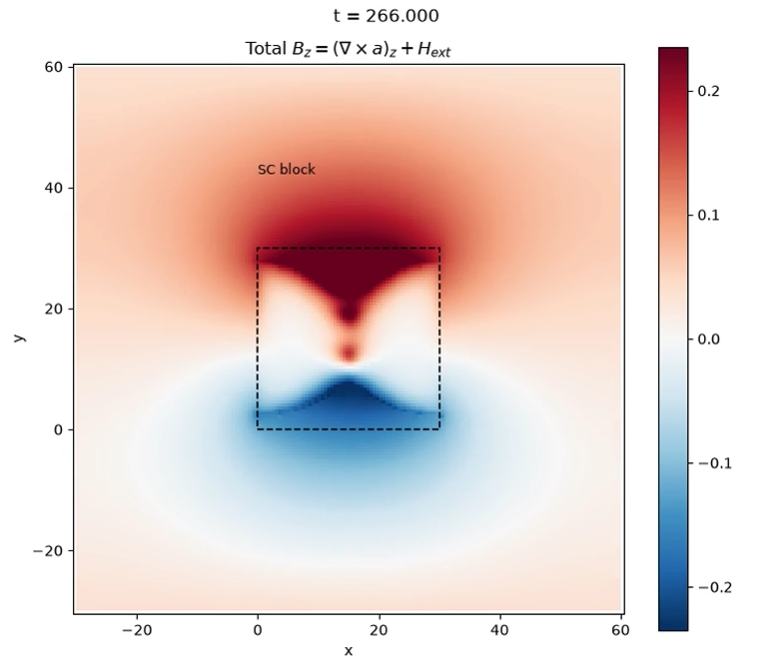
\includegraphics[width=\textwidth]{photos/curlA-no-fix.png}
        \caption{The magnetic field has a hint of red around the vacuum domain because that is just the applied magnetic field. The induced field is significantly larger than the applied field because the current crowding at the constrictions increases current density, thereby increasing $\nabla \times B$ according to Ampere's Law.}
        \label{fig:curlA-nofix}
    \end{subfigure}
    \hfill
    \begin{subfigure}{0.48\textwidth}
        \centering
        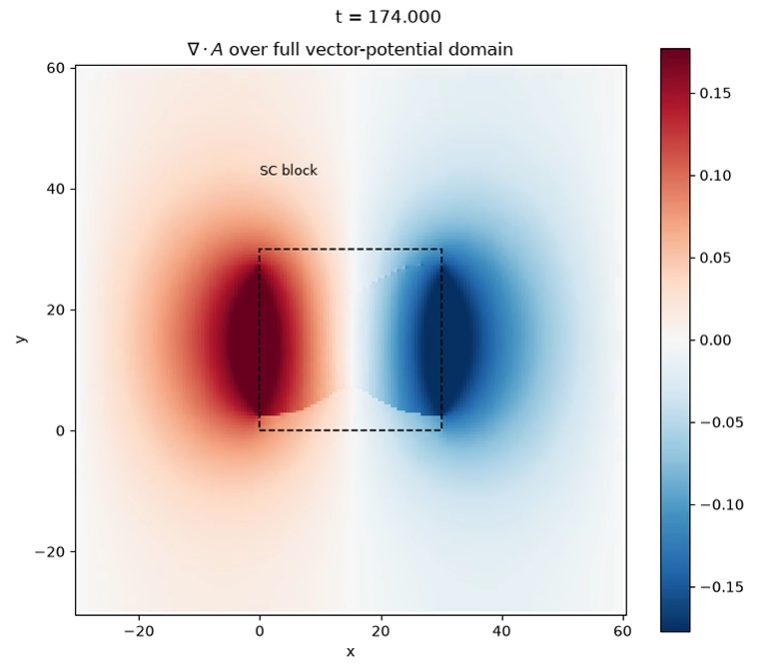
\includegraphics[width=\textwidth]{photos/divA-no-fix.png}
        \caption{This snapshot highlights the large amount of $\nabla \cdot A$ forming the current injection sites. The previous paragraph explains this phenomenon, but as you can tell, $\nabla \cdot A$ is spreading into the SC domain, which can scramble the accuracy of the physics of our simulation.}
        \label{fig:divA-nofix}
    \end{subfigure}
    \caption{Snapshots of the magnetic field ($\nabla \times A$) and $\nabla \cdot A$ over the entire vacuum domain without the fix applied.}
    \label{fig:nofix}
\end{figure}

How did I deal with this? Well, if the problem is with the SC domain and vacuum domain contact where current appears out of nowhere, why not make it so that current doesn't just show up in the middle of the simulation, but was always there? So what I did was extend the $\nabla \phi$ (electric field) to the edge of the vacuum domain so that the current doesn't just show up in the middle of the simulation.

\begin{figure}[htbp]
    \centering
    \begin{subfigure}{0.48\textwidth}
        \centering
        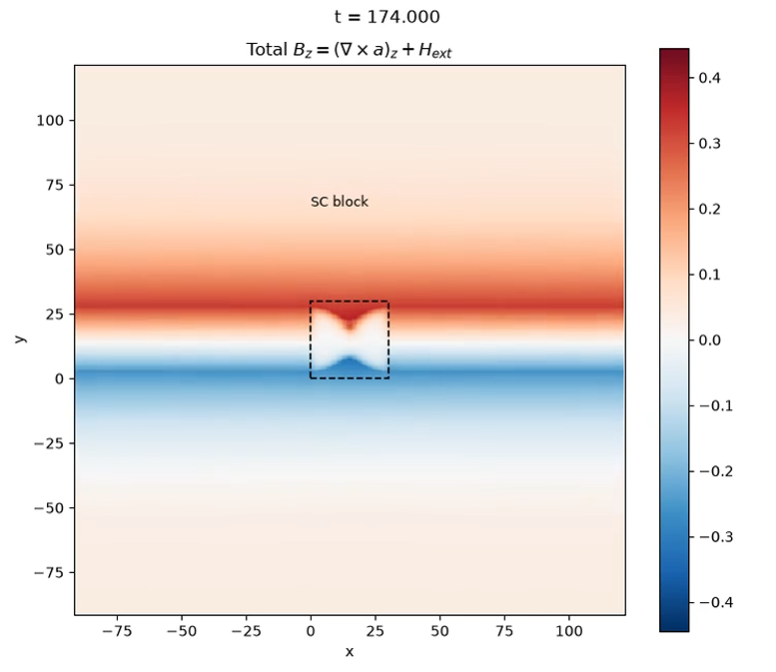
\includegraphics[width=\textwidth]{photos/curlA-fix.png}
        \caption{I previously mentioned the fix for the $\nabla \cdot A$ problem was to create a $\nabla \phi$ stretching to the vacuum domain boundary and, as a result, a current. What's happening here is like there is a normal wire with a constant electric field attached to the superconductor. The red and blue regions at the top and bottom are just the magnetic fields that are induced by current flowing through a wire.}
        \label{fig:curlA-fix}
    \end{subfigure}
    \hfill
    \begin{subfigure}{0.48\textwidth}
        \centering
        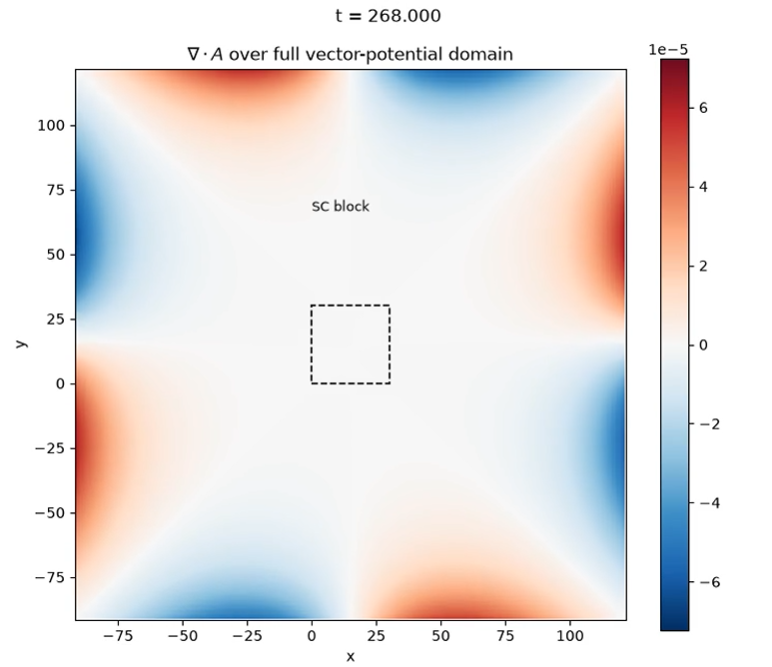
\includegraphics[width=\textwidth]{photos/divA-fix.png}
        \caption{Previously $\nabla \cdot A$ mainly concentrated around the current injection sites and now it's only around the vacuum domain boundaries. It's also about 4 orders of magnitude smaller and doesn't exist anywhere within the SC domain. The largest problem was the existence of $\nabla \cdot A$ in the SC domain, as the Coulomb gauge is required to derive the Poisson equation and the Ampere's Law time step equation. If enough $\nabla \cdot A$ existed in the SC domain, our equations and simulation would have wrongly represented the physics.}
        \label{fig:divA-fix}
    \end{subfigure}
    \caption{Snapshots of the magnetic field ($\nabla \times A$) and $\nabla \cdot A$ over the entire vacuum domain with the fix applied.}
    \label{fig:fix}
\end{figure}

\subsection{Link Variables}
\label{sec:link-variables}

You might be wondering what link variables are. Well, there are some references you can take a look at that I will list~\cite{gropp1996, du2005}, but I can write a quick proof that shows link variables are equivalent to the gauge-covariant derivative.

\begin{equation}
\label{eq:link-claim}
\frac{U_x \psi_{x+1} - \psi_x}{h} \overset{?}{=} (\partial_x - i A_x) \psi_x
\end{equation}

So I need to show this is true where $U = e^{-i \int_x^{x+1} A_x \, dx} \approx e^{-i A_x h}$.

\begin{align}
\psi_{x+1} &= \psi_x + \partial_x \psi_x h \qquad e^{-i A_x h} \approx 1 - i A_x h \label{eq:link-expand}\\
U_x \psi_{x+1} &\approx (\psi_x + \partial_x \psi_x h)(1 - i A_x h) \label{eq:link-prod}\\
&= \psi_x + \partial_x \psi_x h - i A_x \psi_x h - i A_x\partial_x \psi_x h^2 \label{eq:link-prod-2}
\end{align}

Since $h^2$ is small, we can just set it to 0.

\begin{align}
\frac{U_x \psi_{x+1} - \psi_x}{h} &\approx \frac{\psi_x + \partial_x \psi_x h - i A_x \psi_x h - \psi_x}{h} \label{eq:link-final-1}\\
&= \frac{\partial_x \psi_x h - i A_x \psi_x h}{h} \label{eq:link-final-2}\\
&= \partial_x \psi_x - i A_x \psi_x \label{eq:link-final-3}\\
&= (\partial_x - i A_x) \psi_x \label{eq:link-final-4}
\end{align}

\subsection{Current Injection}
\label{sec:current-injection}

The current injection boundary condition is given by the equation $\sigma_n \nabla \phi = J_{\mathrm{inj}}$. Where $J_{\mathrm{inj}}$ is the dimensionless injected current density I use in the code.

Let's discretize this.

\begin{align}
\frac{\phi_{i+1} - \phi_i}{h} &= \frac{J_{\mathrm{inj}}}{\sigma_n} \label{eq:ci-1}\\
\phi_{i+1} = \frac{J_{\mathrm{inj}} h}{\sigma_n} + \phi_i \qquad &\phi_{i-1} = \phi_{i} - \frac{J_{\mathrm{inj}} h}{\sigma_n} \label{eq:ci-2}
\end{align}

With this equation I can put this into the Poisson solver like so. Let $b$ be defined as the RHS of the Poisson equation.

\begin{align}
\nabla^2 \phi = b &= \frac{\phi_{i+1} - 2 \phi_i + \phi_{i-1}}{h^2} \label{eq:ci-poisson-1}\\
\phi_{i+1} - 2 \phi_i + \phi_{i-1} &= b h^2 \label{eq:ci-poisson-2}
\end{align}

For the right side boundary, you can substitute $\phi_{i+1}$ and for the left side substitute $\phi_{i-1}$.

\begin{align}
\frac{J_{\mathrm{inj}} h}{\sigma_n} + \phi_i - 2 \phi_i + \phi_{i-1} &= b h^2 \label{eq:ci-sub-1}\\
-\phi_i + \phi_{i-1} &= b h^2 - \frac{J_{\mathrm{inj}} h}{\sigma_n} \label{eq:ci-sub-2}
\end{align}

Notice the LHS is also conveniently my Neumann boundary condition for non-injection nodes. Since this is the case, all I have to do in the code is add this term $\pm \frac{J_{\mathrm{inj}} h}{\sigma_n}$ onto the RHS of the Poisson solver, where you have minus for the right injection side and plus for the left injection side if you want current to flow from left to right. In the code, $b$ is called src.

\subsection{Staggered Grid: Face vs. Node Quantities}
\label{sec:staggered-grid}

The use of a staggered grid prevents a catastrophic error in my supercurrent and divergence calculations. In my code, all vector quantities reside on the staggered grid and are treated as face values, while scalars are treated as nodal values. But what even are nodal and face values? Each grid point is a node, and imagine a square around that node. Each side of the square is a face, and on those faces reside the vectors, such as the current and the vector potential~\cite{kao2025, coskun1997}.

Time to talk about that catastrophic error caused by treating supercurrents as nodal values. This means taking central differences instead of one-sided differences.

\begin{align}
J_s &= \Im\!\left\{ \psi^*_i \frac{U_i \psi_{i+1} - U^*_{i-1} \psi_{i-1}}{2h} \right\} \label{eq:node-1}\\
&= \frac{1}{2h} \big( \Im\!\left\{ \psi_i^* U_i \psi_{i+1} \right\} - \Im\!\left\{ \psi_i^* U^*_{i-1} \psi_{i-1} \right\} \big) \label{eq:node-2}\\
&= \frac{1}{2h} \big( \Im\!\left\{ \psi_i^* U_i \psi_{i+1} \right\} + \Im\!\left\{ \psi_{i-1}^* U_{i-1} \psi_i \right\} \big) \label{eq:node-3}\\
&= \frac{1}{2h} \big( h g_{i+\frac{1}{2}} + h g_{i-\frac{1}{2}} \big) \label{eq:node-4}
\end{align}

Where $g$ are the face values for supercurrent between nodes.

\begin{equation}
\label{eq:node-avg}
= \frac{g_{i+\frac{1}{2}} + g_{i-\frac{1}{2}}}{2}
\end{equation}

This equation shows that treating $J_s$ as a nodal value is simply the average of the two adjacent face values of that node, but this isn't where the primary problem lies. Let's take a look at the checkerboard pattern where $g_{i+\frac{1}{2}} = -g_{i-\frac{1}{2}}$.

\begin{align}
\frac{g_{i+\frac{1}{2}} + g_{i-\frac{1}{2}}}{2} &= 0 \label{eq:checker-1}
\end{align}

Even when the two face currents are the complete opposites of each other, averaging them results in a nodal current of 0. This is clearly not true and is one of the fundamental problems of storing currents on nodes. A maximally alternating field maps to 0 on a nodal grid. Even worse, you actually use the divergence of $J_s$ in the Poisson equation~\cref{sec:poisson}~\cref{sec:div-js}, and this divergence is completely blind to the checkerboard current pattern, which also results in a wrong Poisson solve and a wrong $\phi$. This pattern is the null mode for our solve. This essentially allows the checkerboard pattern of supercurrent to form anywhere, as our solver is unaware of its presence.

Now look what happens to the divergence if we store supercurrents on the staggered grid instead of averaging them to get nodal currents. Let's use the previously defined $g_{i \pm \frac{1}{2}}$ and consider the checkerboard or maximally oscillating current once more. The checkerboard pattern will take on a form similar to this $g_{i + \frac{1}{2}} = c(-1)^p$, and we will take its derivative to get $\nabla \cdot J_s$.

\begin{align}
\nabla \cdot J_s &= \frac{g_{i+\frac{1}{2}} - g_{i-\frac{1}{2}}}{h} \label{eq:no-checker-1} \\
&= \frac{c(-1)^p - c(-1)^{p-1}}{h} \label{eq:no-checker-2} \\
&= \frac{c(-1)^p + c(-1)^p}{h} \label{eq:no-checker-3} \\
&= \frac{2c(-1)^p}{h} \label{eq:no-checker-4}
\end{align}

The divergence of $J_s$ isn't 0 when considering a maximally oscillating field. Now that it is detectable, our solver can prevent it.

Now the initial condition doesn't start with the checkerboard pattern, so how can it form in the first place? Well, at the center of vortices and current crowding regions, phases can rapidly change, especially at boundaries, the checkerboard field can form. And when it does, our solver never catches it, leading to the aforementioned consequences.

% ================================================================

\bibliographystyle{unsrtnat}   % numbered, in order of first citation
\bibliography{references}

\end{document}